
%----------------------------------------------------------------------------
\chapter{Preliminaries}
%----------------------------------------------------------------------------


\section{Modeling using graphs}

Structural and behavioral modeling of systems are often done using graphs. 
Graphs are useful abstraction as they are easy to understand, intuitive to use, and lots of existing algorithms can be used to process them. 
As model based approach uses models mostly of graph based formalism, in this section, graph based modeling is presented.

A directed graph consists of a set of nodes and a set of edges, where edges are a tuple of two node: a source-- and target node of that edge. 
Graphs can be extended to make them suitable for modeling:

\begin{itemize}
	\item by nodes having attributes with given values (e.g.\ name)
	\item by edges having labels implying their semantics
\end{itemize}

With this extended graph model, there is also a need to give rules for certain types of models, which is the main purpose of domain modeling.
A \emph{domain model} is a metamodel, defining the restrictions for the graph model of a system, i.e.\ what types of nodes exist, what kind of edges can go from one node to another, or what kind of attributes can

\begin{figure}[h]
	\begin{center}
		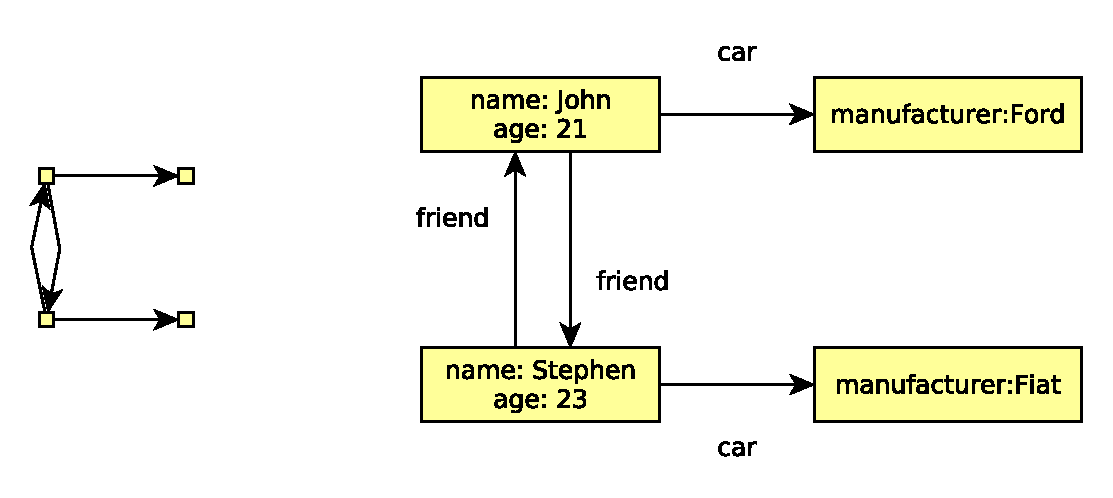
\includegraphics[width=0.75\textwidth]{figures/graphs.pdf}
		\caption{Basic graph (left), and extended (right) }
		\label{fig:graphs}
	\end{center}
\end{figure}


\section{Runtime modeling}

In this framework, we use structural modeling to model the current state of the system. 
This model is called the live model, which captures the state and the operating context of the system. 
We monitor the system through this model: 
The model is updated with sensor data and information from other sources, so the model represents the physical system's latest state. 

\section{Graph pattern matching concepts}

As runtime analysis of the system is based on the runtime model, we needs to identify problems in the graph model. 
Graph pattern matching offers a solution for this task. 
The goal of graph pattern matching is to find all the subgraphs of a graph meeting a certain criteria, defined by a \emph{graph pattern}.

A \emph{graph pattern} is given by a first-order logical expression. 
Not quantified variables are called \emph{parameters}.  
A \emph{pattern match} is a variable binding between parameters and graph vertices, that satisfies the expression.
A \emph{graph query} is a program or execution plan capable of calculating the matches of a graph pattern on a given graph. 
Planning the most efficient graph query is crucial, because the performance of the verification depends on it.



A graph pattern's purpose is to define a list of variables, representing nodes, and a set of constraints for those variables. Some of the possible constraints are:

\begin{itemize}
	\item Type constraint -- a given node must be an instance of a type
	\item Reference -- a given reference must exist between two node
	\item Equality -- two variable must be the same
	\item Inequality -- two variable must have different value
	\item Pattern match -- a subset of variables match to another graph pattern
	\item Negative application condition (NAC) -- a subset of variables must not match to another graph pattern
\end{itemize}
A list of vertices is called a \emph{match}, if binding them to the variables causes the constraints to be true.


\begin{figure}[h]
	\begin{center}
		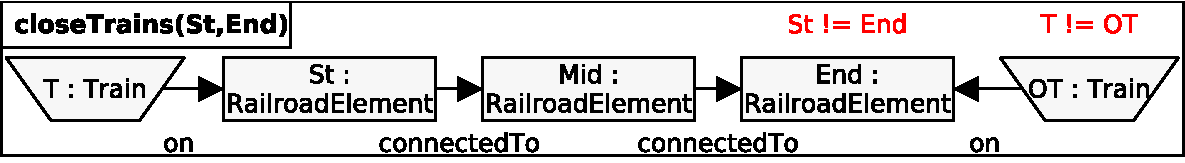
\includegraphics[width=0.75\textwidth]{figures/pattern-visual.pdf}
		\caption{Non-formal visual representation of a graph pattern}
		\label{pattern-visual}
	\end{center}
\end{figure}


\section{Local search}

Local search~\cite{bur-marton-msc} is an algorithm, which provides matchings of a graph pattern in a graph. It is a depth-first search in the space of variable bindings. In the root of the search tree all the variables are unbound. Then with each constraint, we add a new level for the tree. The child of a variable binding is all the other variable binding where 
\begin{itemize}
	\item The bound variables of the parent are bound to the same values as the corresponding variable in the child
	\item The constraint is satisfied by the child
\end{itemize}

The search tree can be traversed without materializing it with depth-first search. This means, that the elements of the search tree are calculated on the fly, by modifying the parent variable binding.

To optimize the size of the search tree the order of the constraints must be chosen properly. 

\section{Distributed platform}

% adatok diszjunkt halmazokra bontva különböző csomópontra
% az algoritmusok is elosztottak, nem lesz összegyűjtve az infó, úgy van kiértékelve, hogy nincs aki mindent látna a rendszerből

As cyber-physical systems are distributed we must deal with the sensor data coming from different sensors at different computation units of the system. Sending the sensor data to one computation unit and evaluate on that cause different problems: Sensor data can be huge to send it through the network, the central node can be a SPOF, etc. In the presented framework the live model is distributed on the different computation units and the graph pattern matching algorithm itself runs in a distributed way. This eliminates the problem of central computers, but introduces complexity, that we must handle. 








